\documentclass{subfiles}
\begin{document}
\begin{wrapfigure}[12]{l}[0pt]{0.4\textwidth}
    \centering
    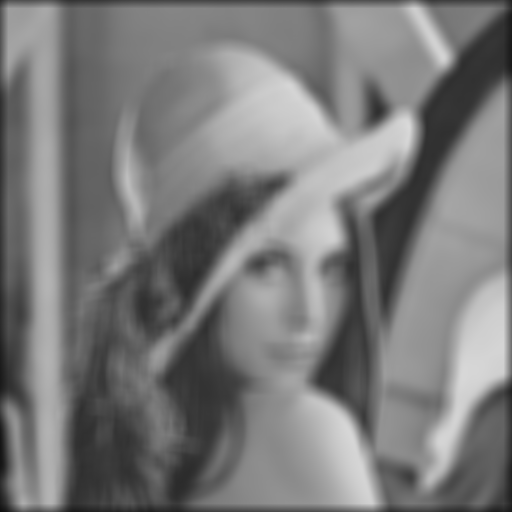
\includegraphics[width = 0.35\textwidth]{../../Figure/Other/Lena/Convolution of Lena with average kernel 21x21.png}
    \caption{Applicazione di un filtro di blur a \emph{Figura \ref{fig:3.1}}.}
    \label{fig:3.2}
\end{wrapfigure}
Il filtro di convoluzione blur permette di applicare una sfocatura all'immagine;
sfocatura che è tanto maggiore tanto maggiori sono i pesi del kernel e le sue dimensioni.
Relativamente al kernel utilizzato, questi è a seguito riportati.
\subfile{../../Figure/Tikz Figure/Snippet convolution.tex}\noindent
Analizzando il codice: \lstinline[language = MATLAB]{fspecial(``type'',``sizes'')} permette di definire un kernel con tipo e dimensioni specificate;
\lstinline[language = MATLAB]{conv2(``base'',``ker'')} effettua la vera e propria convoluzione.  Il perché del parametro ``same'' sarà discusso successivamente.

\end{document}